\documentclass{article}
 
\title{DIY Bike Power}
\author{Demand for Energy Equality}
\date{January 2020 \\ Root source version: Version 1.1 \\ Translation version: Version 0.1}

%inherited code
\usepackage{amsmath,amsthm,amssymb,epsfig}
\usepackage{hyperref}

% imports for images
\usepackage{caption}
% \usepackage[demo]{graphicx}
\usepackage{graphicx}
% \usepackage{float}

% import for resuming enumerated list
\usepackage{enumitem}

% colour import
\usepackage[dvipsnames]{xcolor}

% code to remove numbering but keep the contents page filled
\setcounter{secnumdepth}{0}

\theoremstyle{definition}
\newtheorem{thm}{Theorem}[section]
\newtheorem{lem}[thm]{Lemma}
\newtheorem{prop}[thm]{Proposition}
\newtheorem{cor}[thm]{Corollary}
\newenvironment{pf}{{\noindent\sc Proof. }}{\qed}

\theoremstyle{definition}
\newtheorem*{defn}{Definition}
\newtheorem*{exmp}{Example}
\newtheorem*{prob}{Problem}
\newtheorem*{info}{Information}
\newtheorem*{warn}{Warning}
\newtheorem*{quest}{Question}
\newtheorem*{blockq}{Block Quote}
\newtheorem*{strong}{Strong}
\newtheorem*{code}{Code}
\newtheorem*{coderesult}{Code Result}

\theoremstyle{remark}
\newtheorem*{rem}{Remark}
\newtheorem*{note}{Note}
\newtheorem*{exer}{Exercise}

\setlength{\oddsidemargin}{0.25 in}
\setlength{\evensidemargin}{-0.25 in}
\setlength{\topmargin}{-0.6 in}
\setlength{\textwidth}{6.5 in}
\setlength{\textheight}{8.5 in}
\setlength{\headsep}{0.75 in}
\setlength{\parindent}{0 in}
\setlength{\parskip}{0.1 in}

\hypersetup{
    colorlinks=true,
    linkcolor=black,
    urlcolor=NavyBlue,
    pdfborderstyle={/S/U/W 1}
}

%%%%%%%
% Some commonly used notation
%%%%%%%

\def\R{{\mathbb R}}
\def\X{{\mathcal X}}
\def\Y{{\mathcal Y}}
\def\E{{\mathbb E}}
\def\sign{{\rm sign}}

% END inherited code

\begin{document}
 
\maketitle{}

\begin{center}
  
\includegraphics[width=0.25\paperwidth]{../Images/image_0_0_(demand_energy_equality).png}
\end{center}

\begin{center}
  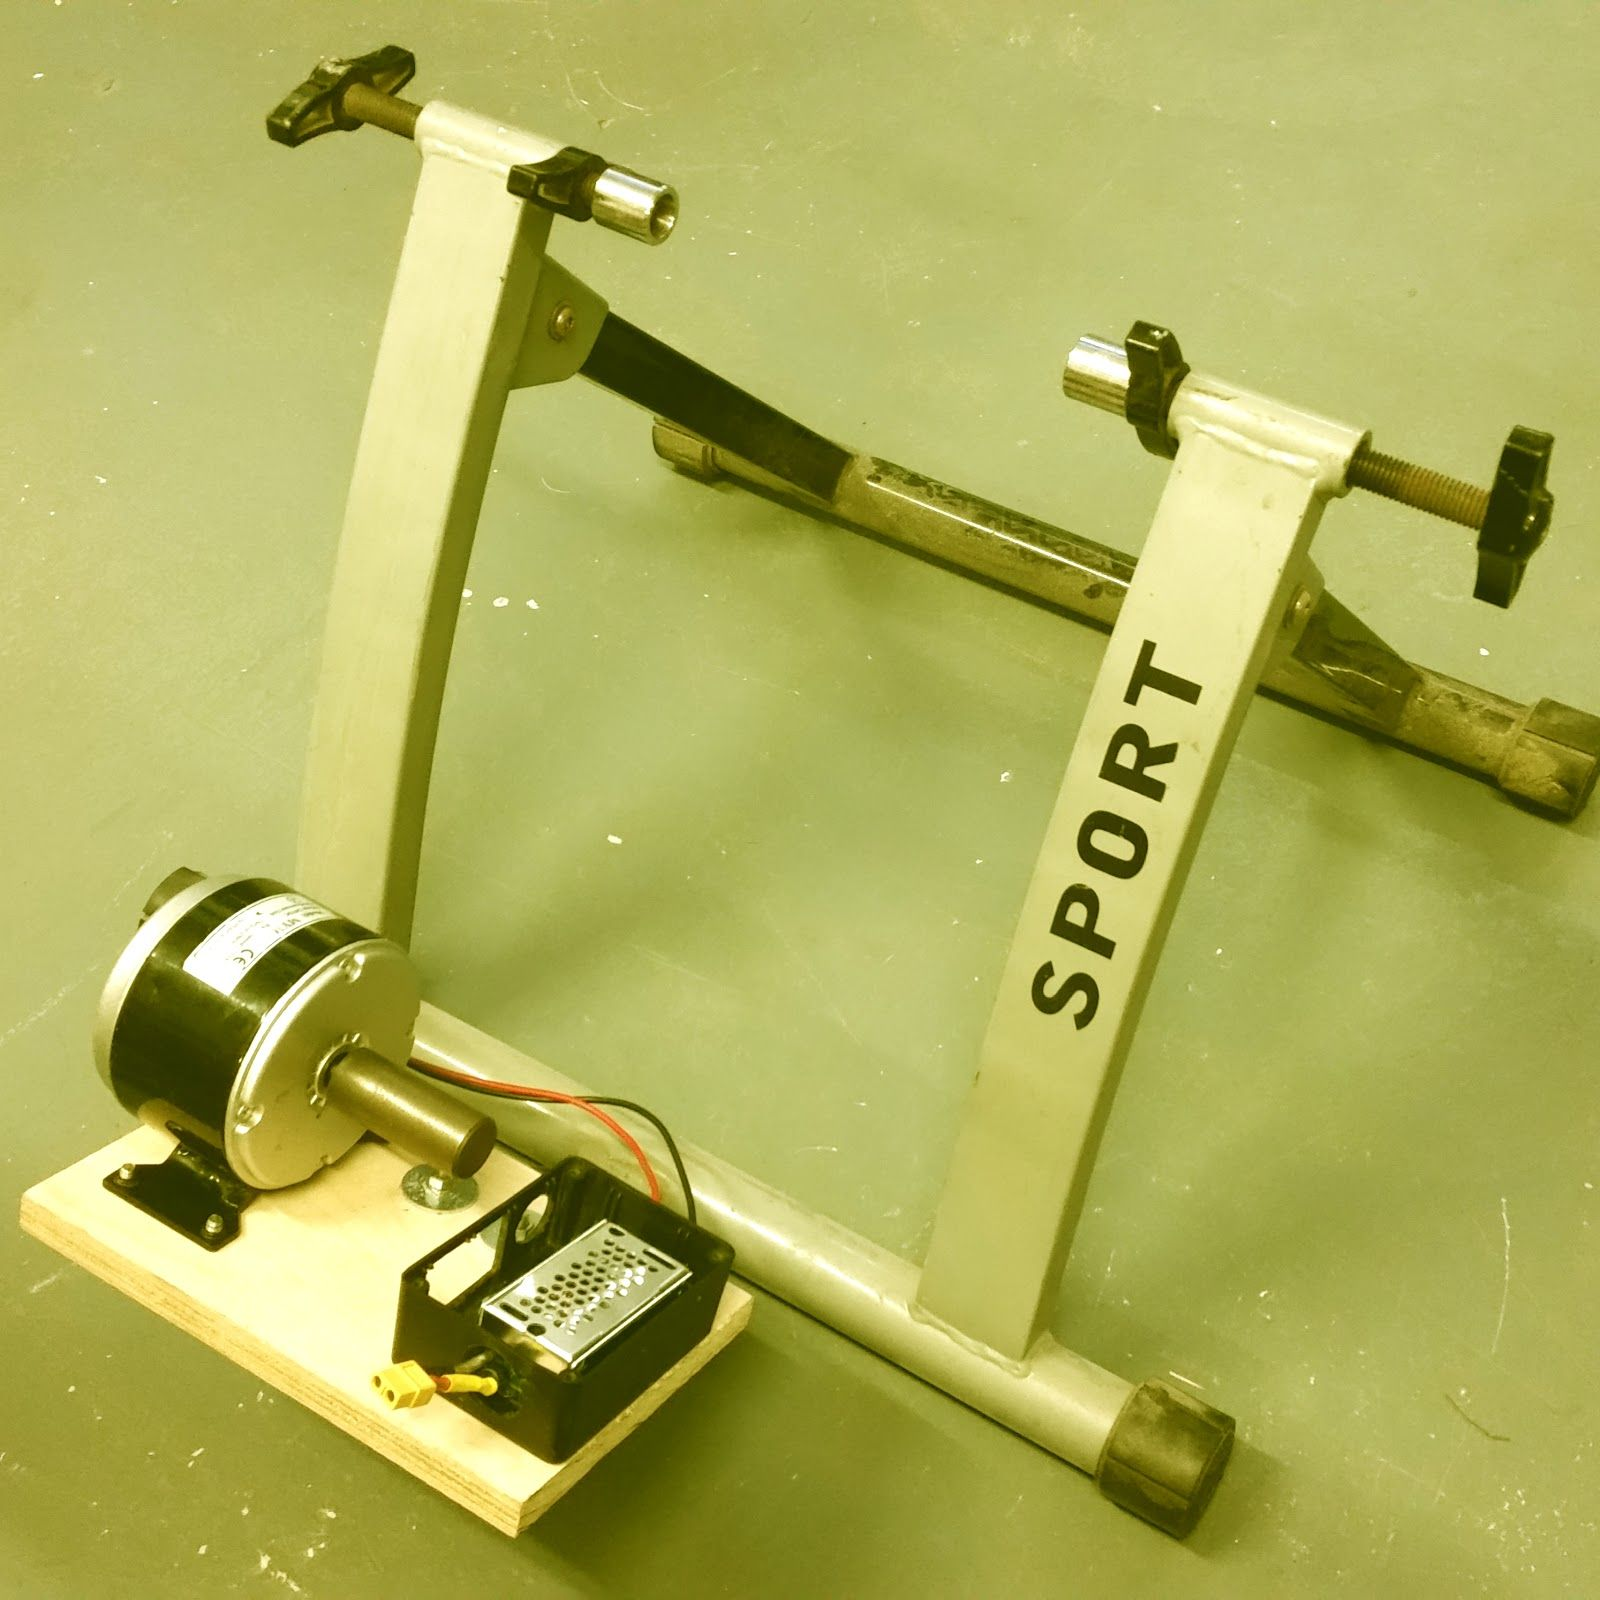
\includegraphics[width=0.45\paperwidth]{../Images/image_0_1_(bike).png}
\end{center}

\vfill
  

\includegraphics[]{../Images/image_0_2_(license).png} \newline
This guide is provided under a \href{https://creativecommons.org/licenses/by-sa/4.0/legalcode}{Creative Commons BY-SA} license: \newline
Material may be freely shared and adapted under the following terms: You must give appropriate credit, provide a link to the license, and indicate if changes were made, and further distribution must be under the same license as the original.

\newpage

\tableofcontents

\newpage

{\color{blue}\section{Preface}} % (fold)
\label{sec:preface}

  \subsection*{Introduction} % (fold)
  \label{sub:introduction}
  
    This PDF has taken the content of the \href{https://www.demandenergyequality.org/build-your-own-bike-generators}{\underline{"DIY Bike Power"}} PDF and put them into a form which can be easily corrected, improved and translated by the community using LaTeX a markdown language for technical topics.

  % subsection introduction (end)

  \subsection*{Notes} % (fold)
  \label{sub:notes}

    Please note the modifications which have been made \& where you can find updates.

    \begin{enumerate}
      \item All the content of the PDF and put them into a form which can be easily corrected, improved and translated by the community using LaTeX a markdown language for technical topics.
      \item Any updates, corrections or translations to the PDF will be available at \href{https://github.com/darigovresearch/DIY-Bike-Power}{\underline{https://github.com/darigovresearch/DIY-Bike-Power}} so do return periodically to check if you have the latest version.
      \item Modifications from the original work includes typo correction, card merging \& consistency consolidation (see the commit history for [en] for the specific changes if any).
    \end{enumerate}

    Feel free to share the PDFs and give the repository a star so more people are likely to see this work and can get the most out of it.

  % subsection notes (end)

  \subsection*{License} % (fold)
  \label{sub:license}

    Unless otherwise specified, everything in this PDF is covered by the following licence:

    
\includegraphics[]{../Images/image_0_2_(license).png} \newline

    This work was based on the work \textbf{\textit{DIY Bike Power}} by \href{https://www.demandenergyequality.org/}{\underline{Demand Energy Equality}}, licensed under a \href{https://creativecommons.org/licenses/by-sa/4.0/legalcode}{\underline{Creative Commons BY-SA}}.

    To see this work in full go to \href{https://www.demandenergyequality.org/build-your-own-bike-generators}{\underline{https://www.demandenergyequality.org/build-your-own-bike-generators}}
  
  % subsection license (end)

% section preface (end)

\newpage

{\color{blue}\section{Introduction}} % (fold)
\label{sec:introduction}

  {\color{blue}\subsection{The Demand Energy Equality project}} % (fold)
  \label{sub:the_demand_energy_equality_project}

    Demand Energy Equality (DEE) is a UK based community energy project that seeks to provide practical energy education, relating mainly to solar generation. We are a group working for systemic change in the way energy is produced, distributed, controlled, delivered and used. These aims are within the context of rising energy inequality (in the UK, at least), rising fuel bills, climate change and the increasing cost of fossil fuel extraction. See \href{https://www.demandenergyequality.org/about/}{\underline{our website}} to find out more about the project.

    Through teaching people hands-on energy skills we also aim to develop their relationship with energy, and enable them to understand it better: where it comes from, how it is used and how it relates to their demand and needs. Ultimately we aim for this to change behaviour, leading to better use of energy and overall reduced demand. Reduced energy use is an unavoidable fact of the relatively near future – far better to prepare now than be surprised later on.

  % subsection the_demand_energy_equality_project (end)
  
  {\color{blue}\subsection{Using this guide}} % (fold)
  \label{sub:using_this_guide}

    This written guide is for anyone interested in building their own basic 12V bike generators, or learning more about the concepts involved. It assumes no prior knowledge of any kind relevant to completing a fully working project. The guide is designed to act as a learning aid for participants on the ‘DIY Bike Power’ workshops run by Demand Energy Equality, and can be used alongside other DIY guides and resources provided by DEE. 

    The guide provides a summary of the concepts involved in energy systems, gives details of a basic bike generator design that can be easily assembled from common components, and explains how you might use bike generators to provide practical energy. Links to useful sources of further research are included at the end of the guide.

    This particular version reflects the most recent iteration of the bike generator design as used by DEE, but it is likely that it may evolve and expand over time. Because we occasionally review and update our content, the guide may not always be in line with the other DIY resources published by DEE, and may not exactly reflect the format of current workshops. Contact DEE if you need an update on any recent changes. 
    
    You will find the latest version of this guide available to download from the DEE website, as and when this guide is updated, alongside our \href{https://www.demandenergyequality.org/resources/}{\underline{other guides and resources}}. Be sure to read the Intro to Off Grid Energy Systems guide for an explanation of basic concepts, and detailed descriptions of charge controllers, batteries, inverters, and other components used in 12V electrical systems.

    For a chance to gain practical experience of the material covered in this guide, please take a look at the \href{https://www.demandenergyequality.org/our-workshops/}{\underline{workshops}} offered on the DEE website.

    We encourage you to share the skills you learn with others through your own workshops, particularly if you are able to target and work with low-income communities. Please contact us for any support you feel you may need if you plan to do this.

  % subsection using_this_guide (end)

  {\color{blue}\subsection{Disclaimer}} % (fold)
  \label{sub:disclaimer}

    This guide is for general guidance only and whilst every effort is made to ensure that the information it contains is correct, it should not be relied upon as accurate. The information / advice contained within this guide is intended for use within the UK only and by persons of no less than 18 years of age. Use this guide at your own risk. DEE will not accept any liability for any loss, damage, injury or negligence direct or indirect from use of the information / advice contained within this guide.

  % subsection disclaimer (end)

  \newpage  

% section introduction (end)

{\color{blue}\section{Before starting}} % (fold)
\label{sec:before_starting}

  {\color{blue}\subsection{Staying safe}} % (fold)
  \label{sub:staying_safe}

    You should be aware of and familiarise yourself with any potential hazards involved in making a bike generator. Ensure you are working in a suitable environment - work indoors on a stable, clear surface, and make sure any trip hazards from trailing cables are cleared away. 

    When working with power tools - drills, jigsaws, etc - always use them properly to avoid the risk of harm or injury. Make sure the tools are all in good working condition, switch off and disconnect tools when not using them, and wear suitable protective equipment (safety glasses, gloves, etc) and avoid loose clothing or accessories that can get caught in moving parts.

  % subsection staying_safe (end)

  {\color{blue}\subsection{Tools and materials}} % (fold)
  \label{sub:tools_and_materials}

    To complete a bike generator you will need: 

    TODO Adjust styling

    \begin{itemize}
      \item a multimeter
      \item a crimp tool
      \item electrical screwdrivers (phillips and flat head, various sizes)
      \item an adjustable spanner or set of spanners
      \item allen keys (various sizes)
      \item wire cutters and strippers
      \item a drill
      \item a ruler or tape measure
      \item wire rated for 10A free
      \item terminal blocks £1
      \item a grey powercon socket £3.50
      \item a project box £6
      \item a 15A step-down buck converter £15
      \item a 10A diode £2
      \item a bicycle training stand £35
      \item a 250W 24V DC electric motor £25
      \item M6 bolts, nuts and washers £1
      \item plywood or metal plate for mounting motor free?
      \item a roller £10
      \item a bicycle (ideally with slick tyres) …?
    \end{itemize}

    Optional:

    \begin{itemize}
      \item a charge controller with a “dump load”
      \item a capacitor rated for 12V with at least 2 Farads capacitance
      \item a 12V lead acid battery
      \item an inverter
      \item In-line fuses
      \item a RCD
      \item an earthing system
      \item cable with blue \& grey powercon plugs
      \item blue powercon socket
      \item a system enclosure e.g. wood box
    \end{itemize}

  % subsection tools_and_materials (end)

% section before_starting (end)

\newpage

{\color{blue}\section{Building a Simple Bike Generator}} % (fold)
\label{sec:building_a_simple_bike_generator}

  Cycle powered generation works by converting the energy supplied by muscles in the human body into electricity. Cycle powered generators use electric DC motors to perform this conversion. Direct drive motors that usually spin when connected to an electrical power supply will have the potential to generate electricity when spun by some other source of power. If you use motors with the right torque and revolution ratio they can be an ideal match up to a person cycling at a steady pace.

  Building and using your own generator requires a number of items. A person, a bicycle, a way of supporting your bicycle off the ground, a motor that can be turned by the bike’s drive system, and a way to regulate the voltage. Each of these parts needs to work efficiently in order to comfortably generate between 50 and 100 watts of usable power from your generator. We will cover each of the parts and how to assemble them into a simple bike generator in this D.I.Y. Guide.

  {\color{blue}\subsection{People}} % (fold)
  \label{sub:people}

    At the end of the day if there are no motivated cyclists you cannot produce electricity. An average person can generate between 40 and 80 watts over extended periods (relatively fit people should be able to produce over 200W in short bursts). You should consider the pedalling speed - most people are most comfortable pedalling at a rate of around 60-80 RPM.
  
  % subsection people (end)

  {\color{blue}\subsection{A Bicycle}} % (fold)
  \label{sub:a_bicycle}

    Of the different types of bicycles used by people to get around, road bikes are most suitable type of bike for generating electricity because they have smooth ‘slick’ tires. Slick tyres help keep friction and noise to a minimum. Road bikes are designed to be efficient on smooth roads. You will generally get more watts from a road bike than a town bike (designed for comfort) or a mountain bike (designed for bumps and jumps).
  
    \subsubsection*{Drive system and gears} % (fold)
    \label{ssub:drive_system_and_gears}

      All bicycles use cogs and a chain to transfer power from the rider to the wheels. This allows the wheels to turn much faster than the rider is pedalling. Bikes with multiple gears have the advantage that they can change the ratio of power transfer, meaning cyclists of different abilities can use them.

      Single speed bikes have the advantage that the cyclist cannot change gear to alter the pedalling speed under high loads. Therefore you can almost guarantee the same power output from each person.

      The ratio of pedalling speed to wheel speed is determined by the ratio of the circumferences of each part. An easy way to calculate this for bike drive systems is to count the teeth on the chainring and cassette. Chainrings (the bit that the pedals are attached to) usually have between 34-50 teeth. Cassettes (the bit that’s on the back wheel) usually have between 12-25 teeth. So the ratio can be between 4.17:1 and 1.36:1.
      This is important for determining the rotational speed of the motor. 

      You should be able to get a good second hand road bike for around £100. A bike with a smaller frame is generally better to use with a bike generator - it’s easier for a tall person to use a bike with a small frame than it is for a short person to use one with a large frame. See Resource 1 for bike projects in London.
    
    % subsubsection drive_system_and_gears (end)
  
  % subsection a_bicycle (end)

  {\color{blue}\subsection{Motors}} % (fold)
  \label{sub:motors}

    We have always used permanent magnet (PM) 24V DC motors in our bicycle generation systems. An electric motor is designed to spin when electricity is passed through it. However, if we use another source of power to spin the motor, the motor will become a dynamo and convert that motion into electrical power. The particular motor we use, which is used a lot of bike generators, is a 24V, 250W scooter motor which is rated at 2750 RPM - part MY 1016 (13.5A) or MY1025 (14A), which you can find on e-bay or other online marketplaces.

    The speed at which the motor is turning (the amount of rotations through 360 degrees undertaken in a set time) normally measured in revolutions per minute (RPM) is directly proportional to (increases and decreases) the voltage output of the pm motor. A motor rated at 2750 RPM and 24V should generate a 12V output when spun at half its rated rotational speed - 1325 RPM.

    Assuming the cyclist maintains a constant pedalling speed, a downhill gear (higher ratio) creates a larger voltage output for the motor than an uphill gear (lower ratio). To maintain the same voltage output when changing gears, the cyclist will need to either increase or decrease their pedalling speed, depending on which gear they change to.

    The torque (rotational force) the cyclist applies to the pedals - normally measured in Newton meters (Nm) - is proportional to the current created by a PM motor. So to generate more current, a cyclist will need to apply more force when pedalling.
      
  % subsection motors (end)

  {\color{blue}\subsection{Rollers}} % (fold)
  \label{sub:rollers}

    The roller attaches to the motor and is turned by the back wheel on the bicycle. Working out what type of roller is suitable is mainly determined by the rotational speed needed by the motor and the size of the wheel on the bike. Adult bike wheels usually have an outside diameter of either 700mm or 26 inches (650mm).

    Attaching a roller to the motor can be quite tricky. We have had some 25mm diameter steel rollers custom made for us, that slide over the motor shaft and are secured in place using a grub screw. These can be made in a metal fabrication workshop with the appropriate metalworking tools. 

    You might find a larger roller (30mm) works better, since it allows a slightly faster pedalling speed. You can also use 52mm skateboard wheels as rollers, that can be mounted onto the motor using a conversion shaft.

    TODO MAKE BOX

    \textbf{Pedalling speed}

    Choosing your bicycle, motor and roller, allows you to determine your pedalling speed. 

    The force from the pedals will be transferred to the motor through the chainring, rear sprocket, back wheel and roller, with the speed determined by the ratio of circumferences of each. With a low gear ratio of 1.36:1, the overall ratio from motor to pedals will be 35.4:1. To maintain a rotational speed of 1325 RPM at the motor, the pedals will need to be rotated at (1325 $\div$ 36.4) 37.5 RPM, or roughly 1 rotation every one and a half seconds, which - while a little on the slow side - is a comfortable pedalling speed.

    \begin{center}
      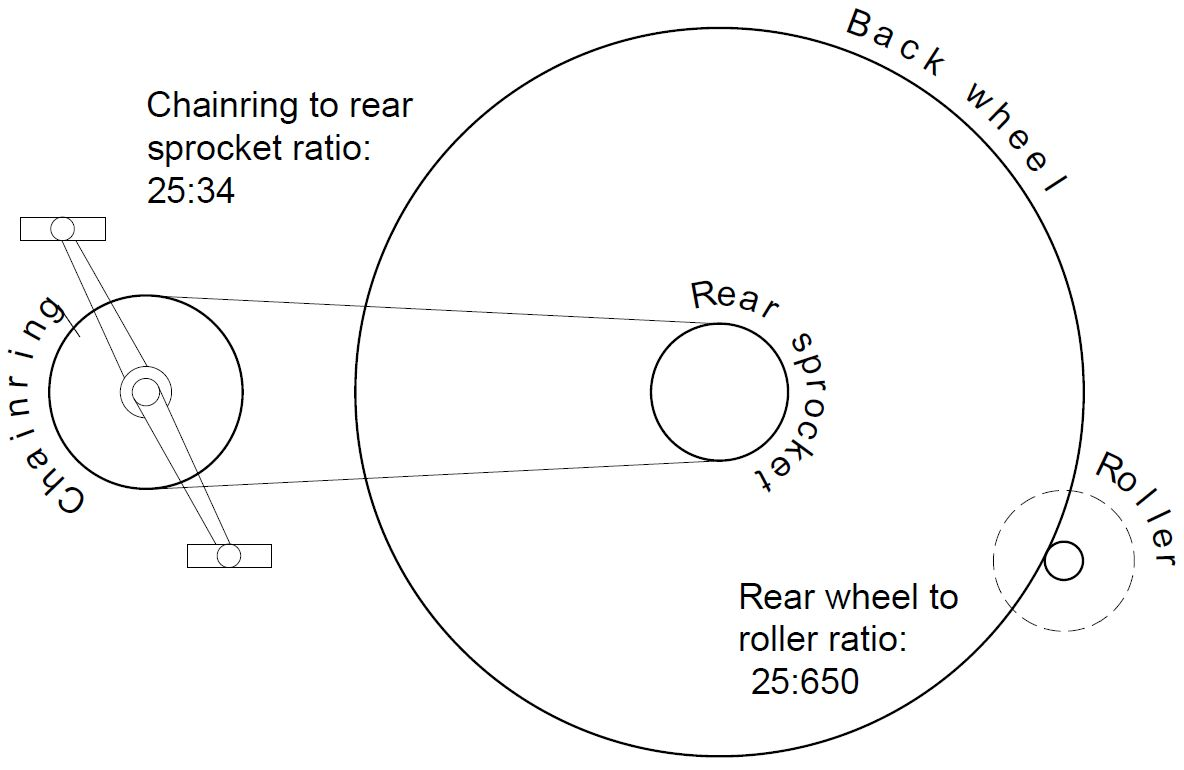
\includegraphics[width=0.35\paperwidth]{Images/image_3_1_(pedalling_speed).png}
    \end{center}
  
  % subsection rollers (end)

  {\color{blue}\subsection{Training stands}} % (fold)
  \label{sub:training_stands}

    We use a training stand (turbo trainer) as a frame for our generator. These can be bought new or second hand from ebay.

    The important thing to look for on a training stand is the tensioning system, which usually holds the resistance roller that is used to provide friction when pedalling. Good ones to look for have the resistance roller mounted on a small metal plate. Removing the resistance roller provides an easy and convenient point to attach the motor and generator assembly onto the training stand. Minoura are a good brand to look for when buying training stands, but other less expensive options exist.

    These training stands tend to fit better on bikes with quick-release rear axles, so if you have a bike that will be used regularly with the bike generator consider fitting one. 

    You could, if you were so inclined, design and build your own bespoke frame and tensioning system, and it’s several examples of bike generator projects using custom stands can be found online to refer to if you want to go down that route, but that approach is not going to be covered in this guide.
  
    \begin{center}
      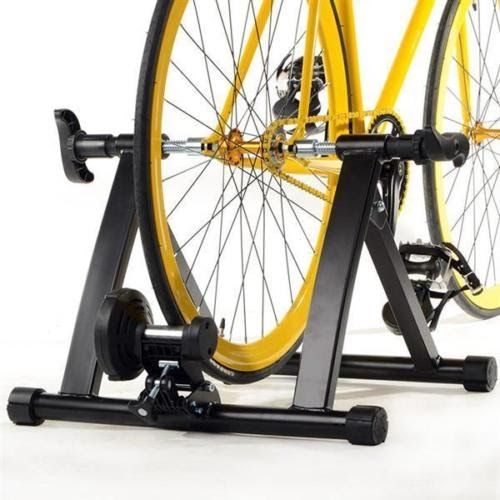
\includegraphics[width=0.25\paperwidth]{../Images/image_3_2_(training_stands).png}
    \end{center}
  
  % subsection training_stands (end)

  {\color{blue}\subsection{Voltage control}} % (fold)
  \label{sub:voltage_control}

    The electrical output from a bike generator with a DC motor tends to be highly variable, since most people do not maintain a constant pedalling speed when cycling. The faster the cyclist pedals, the higher the voltage generated, and there is a tendency for people using bike generators to pedal faster than is needed. There are a number of options for smoothing and controlling the electricity from a bike generator system.

    \subsubsection*{Voltage Regulator Option} % (fold)
    \label{ssub:voltage_regulator_option}

      This option uses a step-down DC to DC Converter to reduce the voltage down to a specified value. The converter can only produce a voltage lower than that supplied to it. So, if you require an output voltage of 12V then the regulator will need to be supplied with a voltage constantly greater than 12V in order to work. The voltage created by the motor in our system is directly proportional to its rotational speed. In order to create a voltage constantly higher than 12V the motor must rotate at a speed of at least 1325 RPM. How fast the motor rotates depend on:

      \begin{itemize}
        \item the speed the cyclist is pedalling (faster = greater motor rpm)
        \item the size of the rear wheel of the bike you are using (larger = greater motor rpm)
        \item what gear the bike is in (downhill/higher gears = greater motor rpm)
      \end{itemize}

      If your appliance or inverter keeps switching on and off when using a DC-DC converter it is usually for one of two reasons.

      \begin{itemize}
        \item the power is being generated at a voltage that is too low (the motor isn't spinning fast enough)
        \item the cyclist is not capable of powering the device you are attempting to power (for a device with variable power levels, this may be monetary - e.g. big bass notes on a sound system)
      \end{itemize}
    
    % subsubsection voltage_regulator_option (end)

    \subsubsection*{Capacitor option} % (fold)
    \label{ssub:capacitor_option}

      \begin{center}
        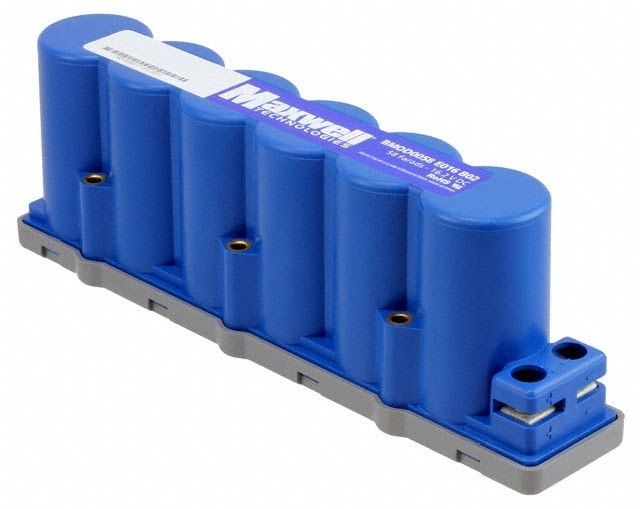
\includegraphics[width=0.15\paperwidth]{../Images/image_3_3_(capacitor_1).png}
      \end{center}

      \begin{center}
        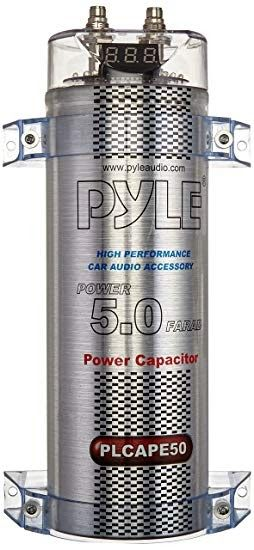
\includegraphics[width=0.10\paperwidth]{../Images/image_3_4_(capacitor_2).png}
      \end{center}

      TODO ADD BOX

      This option uses a very large capacitor, sometimes called a supercapacitor or power capacitor. A capacitor connected in parallel can be used to smooth the variable output voltage from a bike generator, and has the added benefit of providing a short-term energy store to handle load surges. A capacitance of 2 Farad or greater should be adequate for a single generator. Power capacitors which are designed to provide extra bass in a car audio system usually come with a handy voltage display, and can work well in this kind of system.

      Safety note: The types of supercapacitors used in bike generator systems are capable of storing a lot of energy. Because capacitors have zero internal resistance, if a short circuit is created across the positive and negative terminals, all the energy stored in the capacitor will be released at once. This will create a lot of heat, which can cause burns or start fires, and the capacitor itself might explode. This risk is present in even partially charged capacitors, so always make sure to completely discharge a capacitor using a resistor or load before working with it, and after using it.

      A capacitor’s voltage will correspond to the voltage output from the motor, with a smoothing effect on any variation in output that will be more pronounced with a bigger capacitor. If a cyclist is trying to maintain a 12V power supply, they will need to keep an eye on the voltage across the capacitor and adjust their pedalling speed or gear to keep the voltage steady.

      It is possible to over charge a capacitor by applying a high voltage to it. If using an unprotected capacitor you will want to include either a step-down converter or charge controller to limit the voltage going into the capacitor and prevent it from being overcharged should someone decide to pedal very fast.
    
    % subsubsection capacitor_option (end)

    \subsubsection*{Lead Acid Battery Option} % (fold)
    \label{ssub:lead_acid_battery_option}

      In the same way that a capacitor can smooth the voltage output from the motor, a battery can do the same with the added benefit of providing long term energy storage.

      As with capacitors, it is possible to over charge the battery which can result in ‘battery fizz’ - an excess of hydrogen gas. For a 12v lead acid battery the voltage across the terminals should be kept between 12 and 14.5 volts. Batteries with larger capacities are more effective for this purpose - small batteries can be charged or discharged much faster, which can result in fluctuating voltages.

      This option has the potential to quickly ruin a lead acid battery, so you might want to avoid using a high quality expensive battery for this purpose.

      If you want to protect the battery while it is connected to a bike generator, you can use a charge controller. A charge controller monitors the voltage across the battery to ensure that it isn’t too high or that the battery doesn’t become overcharged. You should use a charge controller designed for wind turbines, that will divert power into a dump load when the battery is fully charged. A common charge controller for this is the Morningstar Tristar range. These charge controllers can also be used in combination with a capacitor instead of a battery.

      \begin{center}
        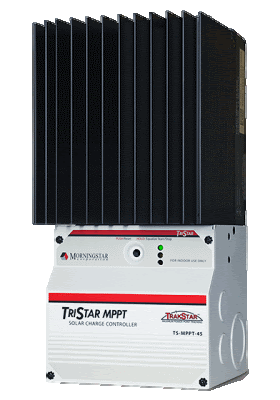
\includegraphics[width=0.10\paperwidth]{../Images/image_3_5_(charge_controller).png}
      \end{center}
    
    % subsubsection lead_acid_battery_option (end)

  % subsection voltage_control (end)

% section building_a_simple_bike_generator (end)

{\color{blue}\section{Assembling the bike generator}} % (fold)
\label{sec:assembling_the_bike_generator}

  The bike generators used by DEE are based on using a step-down converter to regulate the output voltage from the generator. They can be linked together in parallel to charge a capacitor or battery when used to power higher loads.

  The first thing to do is attach the roller to the motor. Our metal rollers slide onto the shaft of the motor and are then fixed in place by tightening a grub screw with a small allen key. 

  Mount the motor and voltage controller on a stiff plywood board or metal plate. The motor has a foot plate with 6mm threaded holes that bolts can be screwed directly into. To protect the voltage regulator, it can be mounted inside a plastic project box or similar enclosure. 

  \begin{center}
    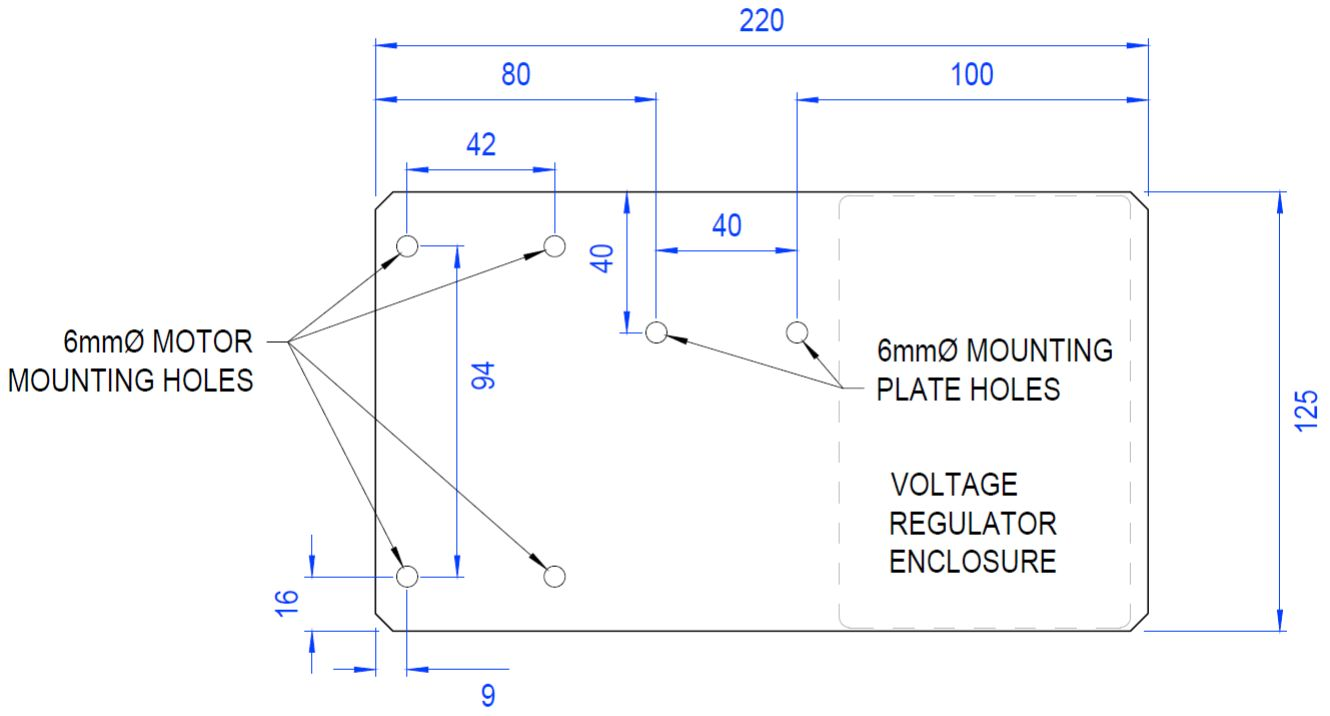
\includegraphics[width=0.75\paperwidth]{Images/image_4_1_(mounting_board).png}
  \end{center}

  The wires from the motor should connect to the input on the voltage regulator. Remember that to generate electricity, the motor will be spun in reverse, so the positive and negative wires should be reversed - the black wire should connect to the positive input and the red wire should connect to the negative input. You will also need to connect a 10A diode to the output to prevent backflow from a capacitor or battery. To make it easy to connect the generator to other devices, it is worth using a standard connector on the output, such as an XT60 or Powercon.

  \begin{center}
    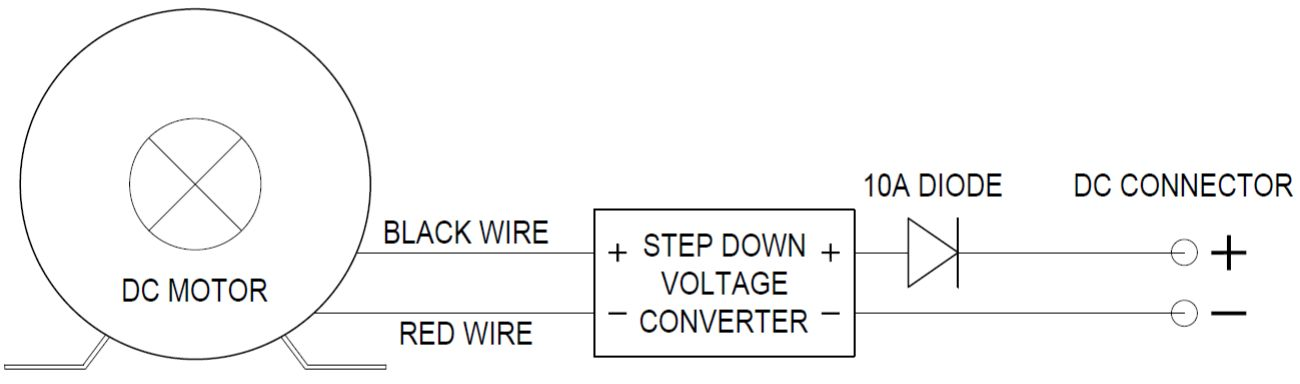
\includegraphics[width=0.75\paperwidth]{Images/image_4_2_(dc_motor).png}
  \end{center}

  The motor/regulator board should be attached the metal mounting plate on the training stand with 6mm bolts. Use large washers to spread the load on a wooden mounting board, and split ring washers to maintain the bolt tightness.

  \begin{center}
    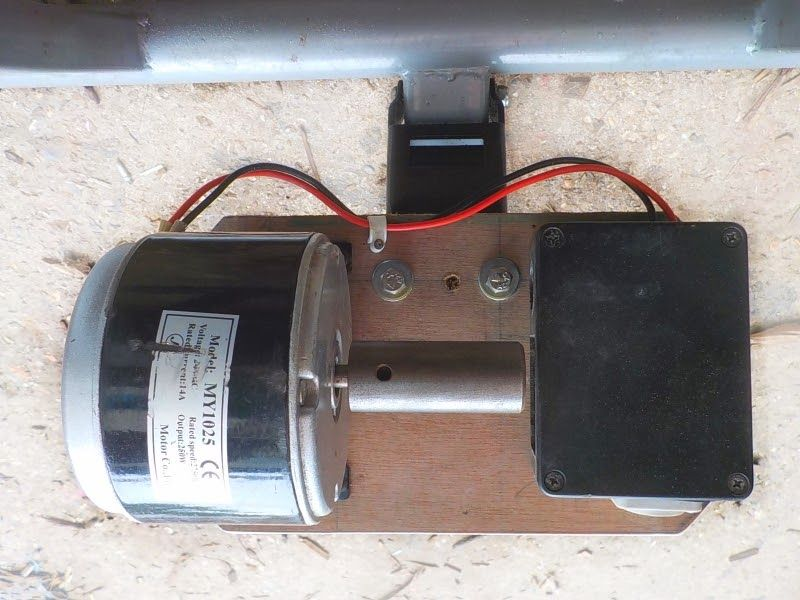
\includegraphics[width=0.45\paperwidth]{../Images/image_4_3_(dc_motor_mounted).png}
  \end{center}

  With a bicycle mounted on the training stand, check the position of the back wheel. It should be located as close to the motor body as possible. You can adjust the axle clamps on the training stand to move the wheel sideways as needed. Once the wheel is in the appropriate position, the mounting plate needs to be tensioned so that it can turn the roller. Turn the tensioning screw under the mounting plate until the roller is pressed firmly against the tyre on the back wheel of your bike. The tighter it is, the less chance of the tyre slipping when turning the roller under high loads, but the more friction will be generated. The exact tightness to use can be found through trial and error - test the generator on the highest load you expect to use, and if there is any slippage, increase the tension slightly and test again until it turns without slipping at all.

  You should now be ready to use the bike generator. You can use it to directly power a variety of 12V appliances - lights, stereo, kettle, phone charging, laptop charging, etc. Bear in mind that the most power you should expect to generate from one bike generator is around 100 Watts.

  \begin{center}
    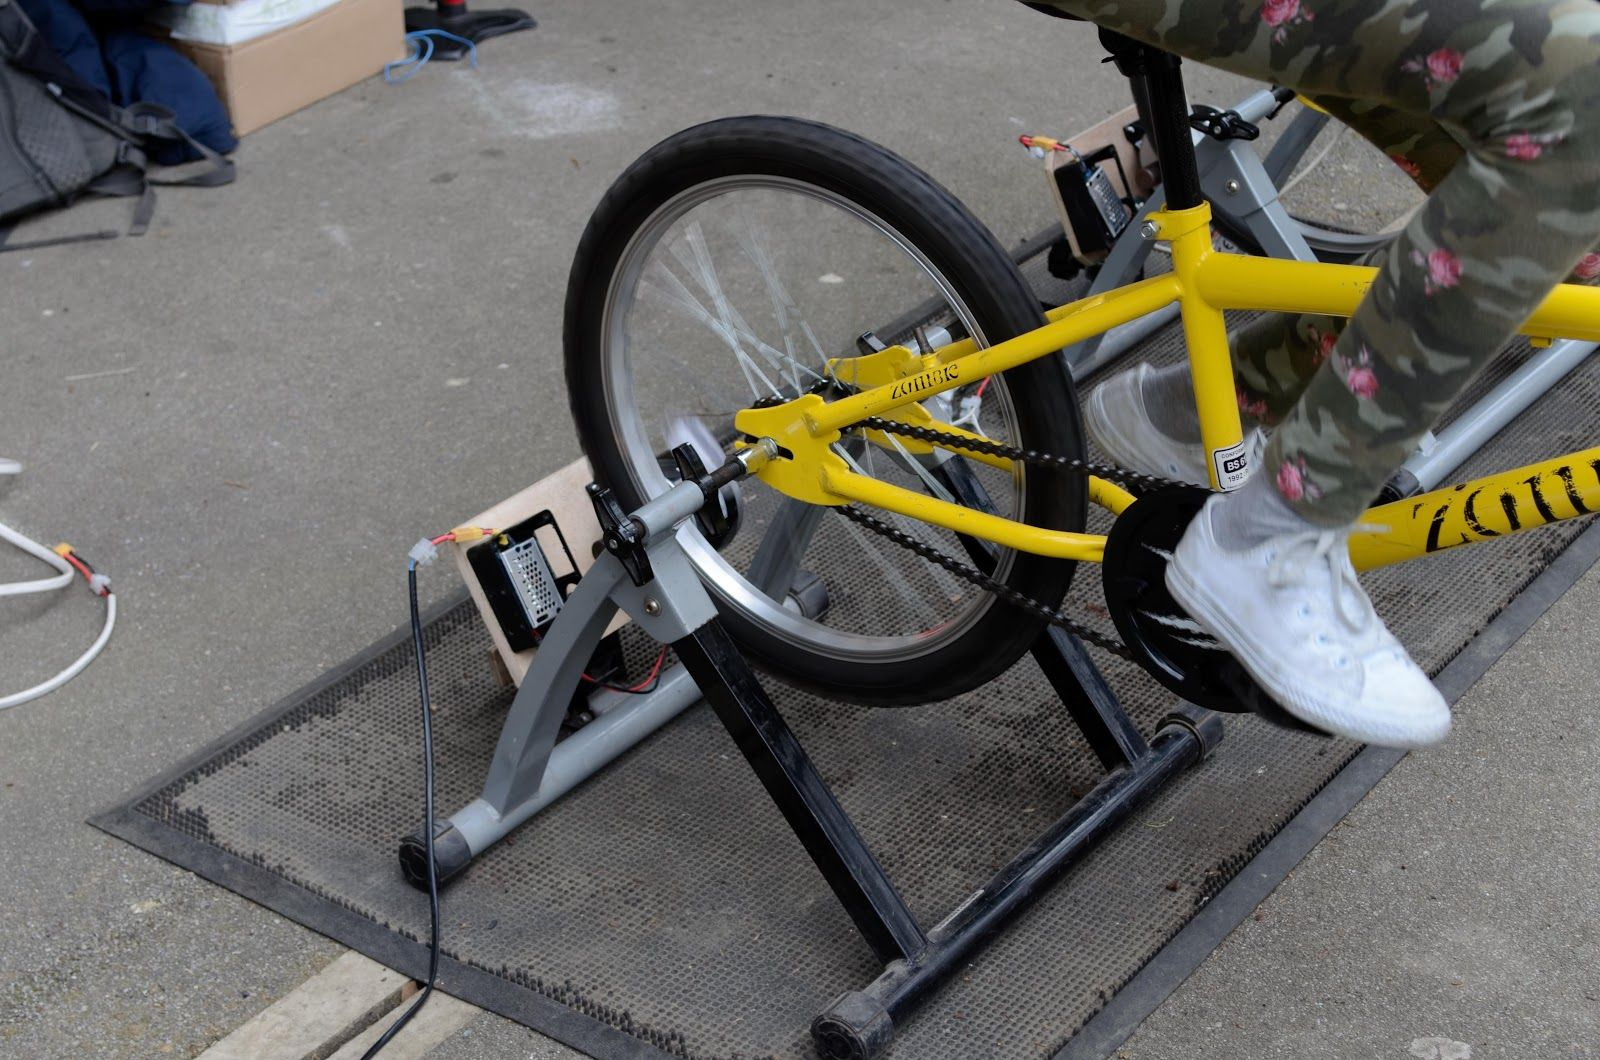
\includegraphics[width=0.45\paperwidth]{../Images/image_4_4_(generator_for_use).png}
  \end{center}

% section assembling_the_bike_generator (end)

{\color{blue}\section{Using multiple bike generators}} % (fold)
\label{sec:using_multiple_bike_generators}

  For loads of more than 100W, you will need to build a system that uses more than one bike generator. If multiple bike generators are being used at the same time, their power can be combined via a distribution board, which can contain all the voltage regulation and system protection components. 

  \begin{center}
    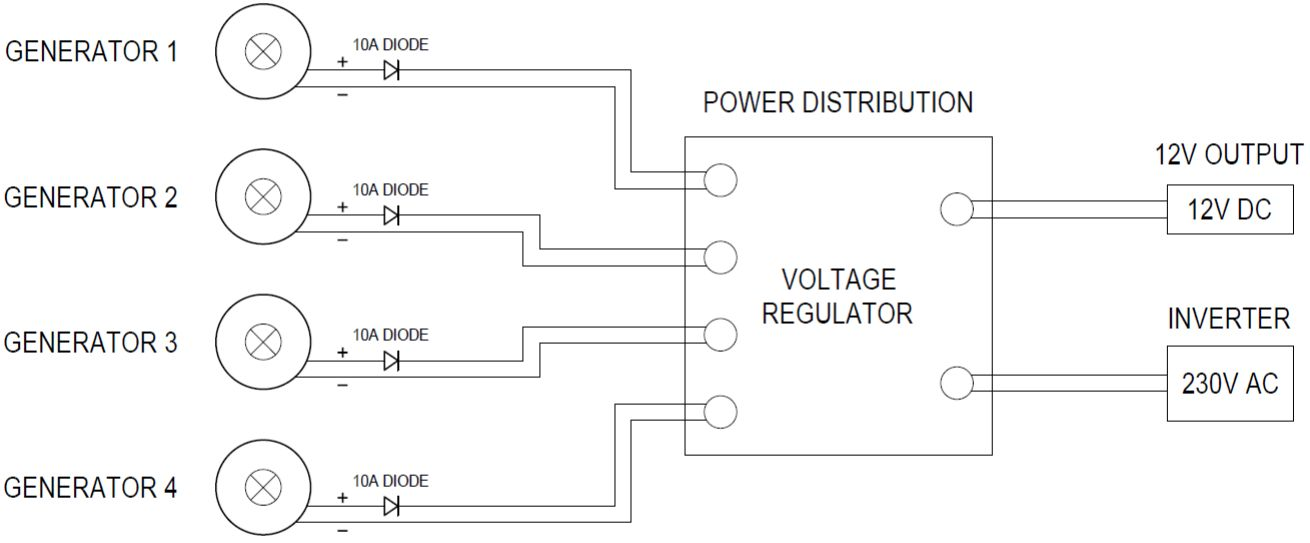
\includegraphics[width=0.75\paperwidth]{Images/image_5_1_(multiple_generator_diagram).png}
  \end{center}

  \subsubsection*{Cables and connectors} % (fold)
  \label{ssub:cables_and_connectors}

    We use 20A Powercon connectors when connecting the bikes into either a multiple or single bike system. The connectors hold a good connection, can be easily connected and disconnected, and are simple to make yourself. You can also use XT60 connectors as a cheaper option, but they are not as robust or easy to use.

    It’s a good idea to get fairly thick, heavy duty wire for your power cables, especially when dealing with long cables (2m or more). Long runs of thin wire will result in significant energy losses - the smaller the wire diameter, the more it heats up when an electrical current is passed through it, and the more energy is lost. Paired (black \& red wires in the same sheath) 4mm 2 (or 2.5mm 2 ) core speaker cable is a good option, which results in a good looking, durable cable.
  
    \begin{center}
      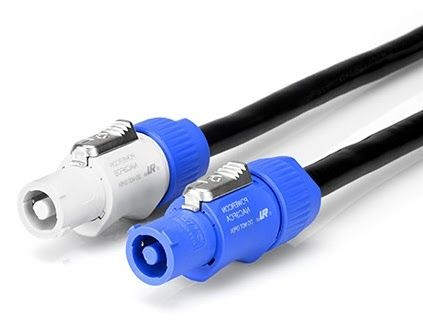
\includegraphics[width=0.15\paperwidth]{../Images/image_5_2_(connectors).png}
    \end{center}

  % subsubsection cables_and_connectors (end)

  \subsubsection*{Inverters} % (fold)
  \label{ssub:inverters}

    If you want to use AC mains powered appliances you will need to use an inverter, which will convert the 12V DC power from your bike generator(s) into 240V AC power. There are two types of inverters: a pure sine wave inverter produces a smooth wave on the AC output, while a modified (or quasi) sine wave produces a stepped square wave. Some devices may not work properly with a modified sine wave inverter.

    Inverters designed to work with 12V batteries will usually work with voltages between 10 and 14 volts, but will work best with a power supply with a voltage of 12-13 volts. If using an inverter, it is highly recommended that you use a large capacitor or battery to maintain a smooth, stable voltage on the power supply to the inverter.
  
    \begin{center}
      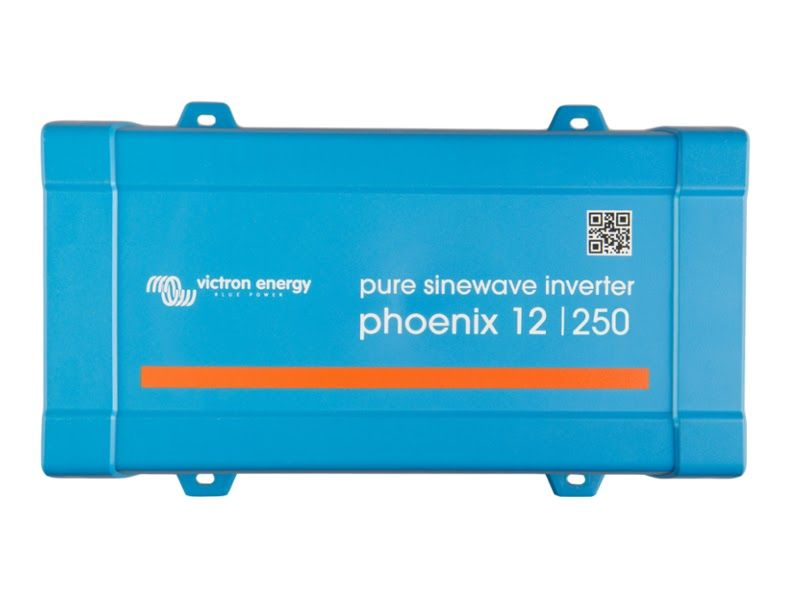
\includegraphics[width=0.15\paperwidth]{../Images/image_5_3_(inverter).png}
    \end{center}

  % subsubsection inverters (end)

  {\color{blue}\subsection{An example of a multi-generator system distribution board}} % (fold)
  \label{sub:an_example_of_a_multi_generator_system_distribution_board}

    The image to the right shows a distribution board for a bike generator system built by \href{https://www.electricpedals.com/}{\underline{Electric Pedals}}.

    It has five blue powercon inputs linked together with bus bars to connect up to five bike generators in parallel. 

    It uses a Maxwell supercapacitor to smooth the power output and provide some energy storage.

    It has a Morningstar charge controller with a large resistor acting as a dump load to regulate the voltage and protect the system against over-voltage. The inverter displays the system voltage to provide feedback to the users.

    The output goes via a Victron inverter connected to regular household 3-pin sockets to provide 230V AC power. 

    Fuses from the power input and to the inverter protect the system against over-current.

    A system like this can be used with unregulated generators, so the power would come directly from the motors without needing to go through a voltage converter. 

    More information on the components used in this system (inverters, fuses, charge controllers, etc) can be found in our \href{https://www.demandenergyequality.org/get-started-with-offgrid}{\underline{Intro to DIY Off Grid Systems}} guide.
    
    \begin{center}
      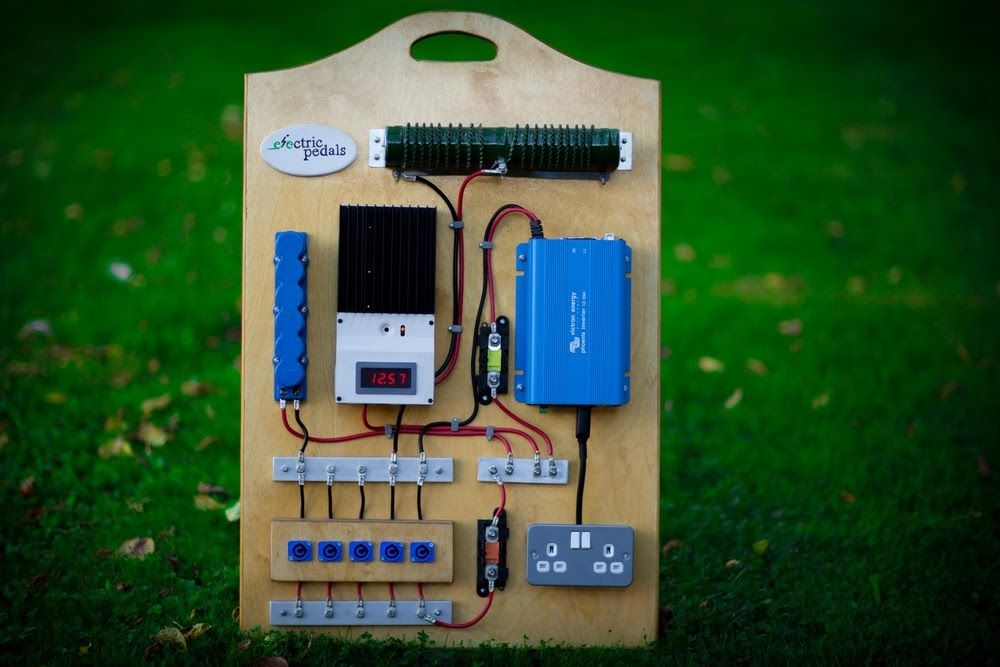
\includegraphics[width=0.35\paperwidth]{../Images/image_5_4_(example_board).png}
    \end{center}

    \begin{center}
      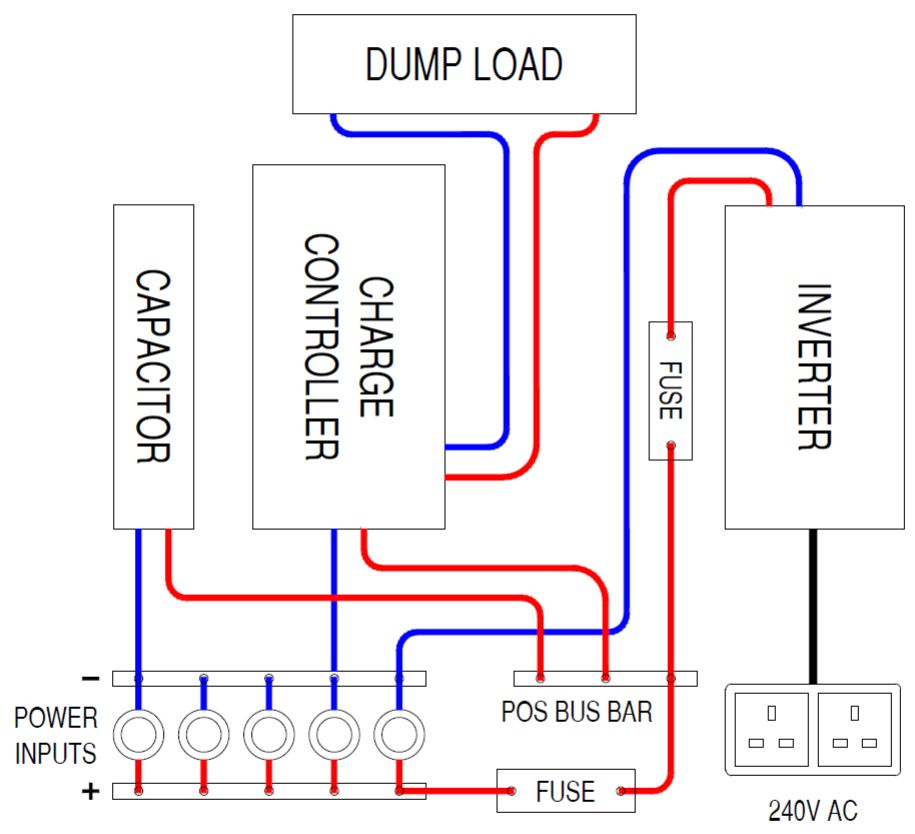
\includegraphics[width=0.35\paperwidth]{Images/image_5_5_(example_diagram).png}
    \end{center}

  % subsection an_example_of_a_multi_generator_system_distribution_board (end)

% section using_multiple_bike_generators_ (end)

{\color{blue}\section{Resources}} % (fold)
\label{sec:resources}

  \begin{enumerate}
    \item Bike projects in London:  \newline
      The Bike Project: \href{https://thebikeproject.co.uk/}{\underline{https://thebikeproject.co.uk/}} \newline
      Brixton Cycles Co-op: \href{http://www.brixtoncycles.co.uk/}{\underline{http://www.brixtoncycles.co.uk/}} \newline
      London Bike Kitchen: \href{https://lbk.org.uk/}{\underline{https://lbk.org.uk/}} \newline
    \item There are a number of other methods for building bike generators using car alternators or stepper motors. See \href{http://www.scienceshareware.com/}{\underline{http://www.scienceshareware.com/}} \newline
      Here’s another design that uses the weight of the motor to maintain contact between the back wheel and the roller: \href{http://www.appropedia.org/Rowan\%27s\_portable\_pedal\_power\_generator}{\underline{http://www.appropedia.org/Rowan\%27s\_portable\_pedal\_power\_generator}}
    \item Cycle powered generation: \href{http://www.stewardwood.org/resources/DIYcyclepower.htm}{\underline{http://www.stewardwood.org/resources/DIYcyclepower.htm}}
    \item How a lead acid battery works: \href{http://www.progressivedyn.com/battery_basics.html}{\underline{http://www.progressivedyn.com/battery\_basics.html}}
    \item Calculating line losses: A handy calculator to help you work out losses over distance for different thickness of wire. \href{http://www.solar-wind.co.uk/cable-sizing-DC-cables.html}{\underline{http://www.solar-wind.co.uk/cable-sizing-DC-cables.html}}
  \end{enumerate}

  \subsection{Bike Generator Providers} % (fold)
  \label{sub:bike_generator_providers}
  
    \begin{enumerate}[resume]
      \item Reaction Bike Power: \href{https://bike-power.co.uk/}{\underline{https://bike-power.co.uk/}}
      \item V3 Power: \href{http://v3power.co.uk/bicycle-generators/}{\underline{http://v3power.co.uk/bicycle-generators/}}
      \item Electric Pedals: \href{https://www.electricpedals.com/bicycle-friction-generator/}{\underline{https://www.electricpedals.com/bicycle-friction-generator/}}
    \end{enumerate}
  
  % subsection bike_generator_providers (end)

  \subsection{Other Renewable Energy Resources} % (fold)
  \label{sub:other_renewable_energy_resources}

    \begin{enumerate}[resume]
      \item Introduction to DIY Off Grid Energy systems: \newline
        \href{https://www.demandenergyequality.org/get-started-with-offgrid}{\underline{https://www.demandenergyequality.org/get-started-with-offgrid}}
      \item DIY solar panels: \href{https://www.demandenergyequality.org/build-your-own-panels}{\underline{https://www.demandenergyequality.org/build-your-own-panels}}
      \item How solar cells work: \href{https://www.demandenergyequality.org/guide-to-solar-energy}{\underline{https://www.demandenergyequality.org/guide-to-solar-energy}}
      \item DIY wind turbines: \newline
        V3 Power run courses: \href{http://v3power.co.uk/}{\underline{http://v3power.co.uk/}} \newline
        Hugh Piggott Designs: \href{http://scoraigwind.co.uk/}{\underline{http://scoraigwind.co.uk/}}
      \item DIY micro hydro:  \href{http://www.stewardwood.org/resources/hydroelectric.ghtml}{\underline{http://www.stewardwood.org/resources/hydroelectric.ghtml}} \newline
        \href{https://www.permaculture.co.uk/articles/310505923/building-your-own-renewable-energy-systems-recycled-materials}{\underline{https://www.permaculture.co.uk/articles/310505923/building-your-own-renewable-energy-systems-recycled-materials}}
      \item Renewable energy diagram by Merlin Howse: \newline
        \href{http://offthegrid.org.uk/resources/renewable-energy-diagram-2.0.pdf}{\underline{http://offthegrid.org.uk/resources/renewable-energy-diagram-2.0.pdf}}

    \end{enumerate}
  
  % subsection other_renewable_energy_resources (end)

  \subsection{Off grid system component suppliers} % (fold)
  \label{sub:off_grid_system_component_suppliers}

    \begin{enumerate}[resume]
      \item Wind and Sun: \href{http://www.windandsun.co.uk/}{\underline{http://www.windandsun.co.uk/}}
      \item Bimble Solar: \href{http://www.bimblesolar.com/}{\underline{http://www.bimblesolar.com/}}
    \end{enumerate}
  
  % subsection off_grid_system_component_suppliers (end)

% section resources (end)

\newpage

{\color{blue}\section{Appendix}} % (fold)
\label{sec:appendix}

  {\color{blue}\subsection{Equipment List}} % (fold)
  \label{sub:equipment_list}

    \textbf{Equipment – Bike generator}
    Motor \newline
    Training stand \newline
    Voltage regulator \newline
    Bicycle \newline
    12V to USB converter \newline
    12V laptop charger \newline
    12V LEDs \newline
    12V amplifier and speakers

    \textbf{Equipment – Tools} \newline
    Multimeter \newline
    Wire strippers \newline
    Wire cutters \newline
    Screwdrivers \newline
    Spanners \newline
    Crimping tool \newline
    Allen keys \newline
    Drill \newline
    Ruler

    \textbf{Equipment – Distribution} \newline
    Powercon cable and sockets \newline
    Power capacitor / supercapacitor \newline
    Voltmeter \newline
    Switches \newline
    Inverter \newline
    Fuses \newline
    Charge controller \newline
    Dump load resistor
  
  % subsection equipment_list (end)

  {\color{blue}\subsection{Using a Multimeter}} % (fold)
  \label{sub:using_a_multimeter}

    \begin{center}
      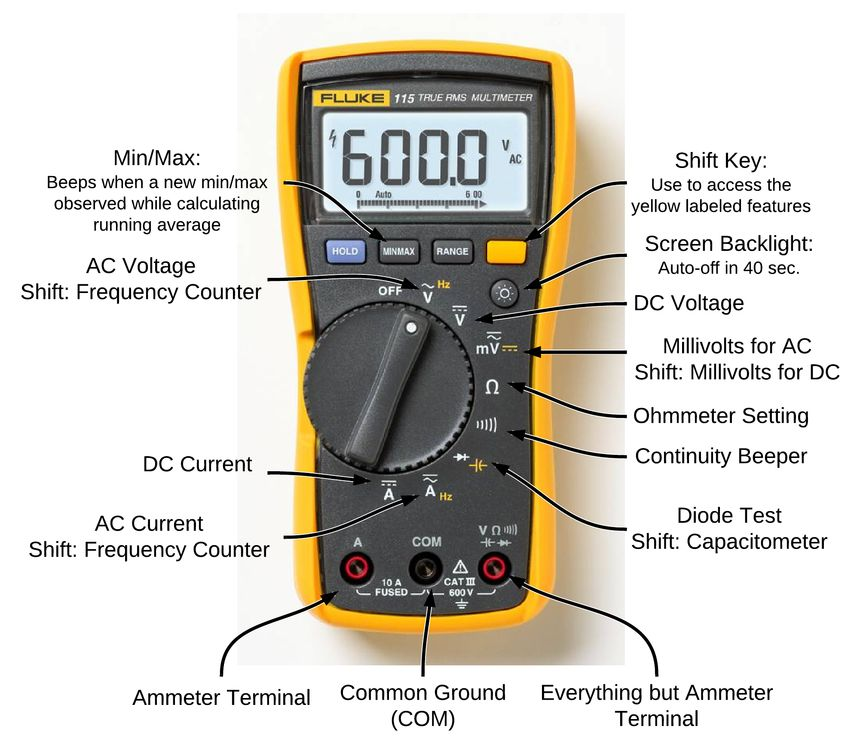
\includegraphics[width=0.45\paperwidth]{Images/image_a_1_(multimeter).png}
    \end{center}
  
  % subsection using_a_multimeter (end)

% section appendix (end)

\end{document}